

\chapter{Random Process}

In this chapter, we see how to generate white noise with correct PSD.\\


Assuming a baseband model of bandwidth $B$ Hz, and AWGN channel, the total noise power is the area

\begin{figure}[h]
\centering
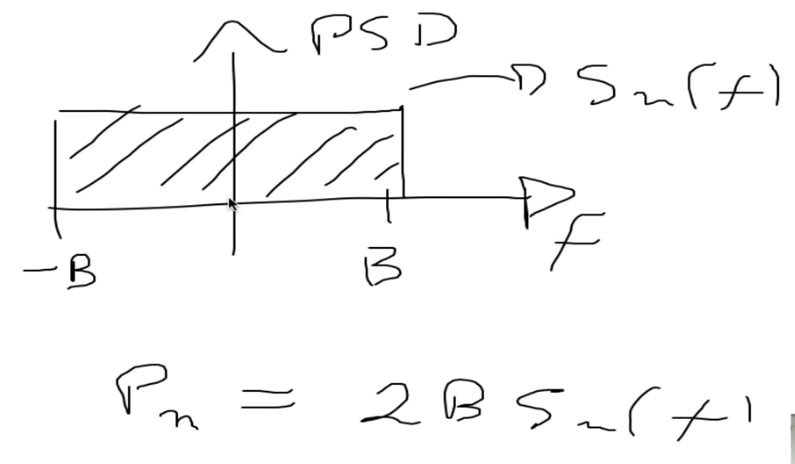
\includegraphics[scale = 0.5]{Figures/Random_Process/Total_Noise_Power_AWGN}
\caption{PSD for AWGN Baseband Model}
\label{fig:Random_Process_Total_Noise_Power_AWGN}
\end{figure}

From random process, the power of random sequence $X[n]$ is equal to the mean square, that is $E[X^2]$.

Now if this sequence have zero mean, then the mean square will be equal to the variance $\leftrightarrow \, E[X^2] \, = \, \sigma$.

So if want to generate some  noisy sequence having some total power (whih is equal to $\sigma$), we simply multiply the noisy sequence generated with the standard deviation $\sqrt{\sigma} \leftrightarrow \, $ 


%*****************************************************
%*****************************************************
%*****************************************************